\chapter{الإعدادات المحلية وميزات إضافية}
\label{ch:04-features}

\section{اضبط اللغة والتقويم}
\label{sec:features-regional}

تعتمد التواريخ والمواعيد والرسائل على إعدادات المؤسسة. وإذا تُركت على قيمها العامة، فقد يتأخر موعد عن الدوام الفعلي، أو تصل رسالة بلغة لا يتوقعها الموظف. لذلك اضبطها قبل التجربة، وقبل إطلاق أي خطة.

\begin{rcnote}[مثال: مديرية الواحة]
تعمل المديرية في دمشق، ويبدأ أسبوع عملها يوم الأحد. لذلك تختار المنطقة الزمنية لدمشق، و«الأحد» بداية للأسبوع، والعربية لغة افتراضية.
\end{rcnote}

\begin{figure}[H]
\centering
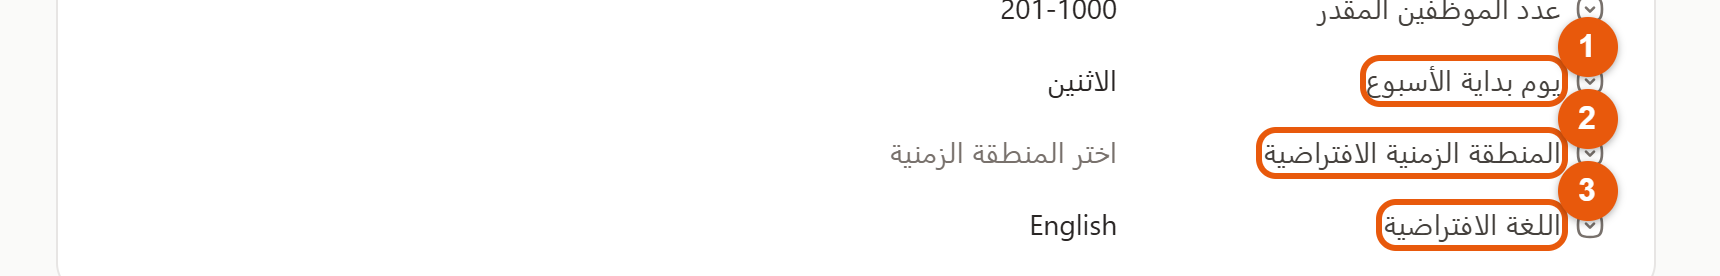
\includegraphics[width=0.85\linewidth]{assets/screens/org-regional.png}
\caption{إعدادات المؤسسة التي تؤثر في التواريخ}
\label{fig:features-regional}
\shotnote{تعرض الصورة قيماً تحتاج إلى مراجعة في مؤسسة عربية: لم تُحدَّد منطقة زمنية، واللغة الافتراضية الإنجليزية. ① «يوم بداية الأسبوع»: اجعله مطابقاً لأسبوع عملكم. ② «المنطقة الزمنية الافتراضية»: اختر منطقة دمشق. ③ «اللغة الافتراضية»: اختر العربية إذا كانت لغة العمل.}
\end{figure}

\begin{figure}[H]
\centering
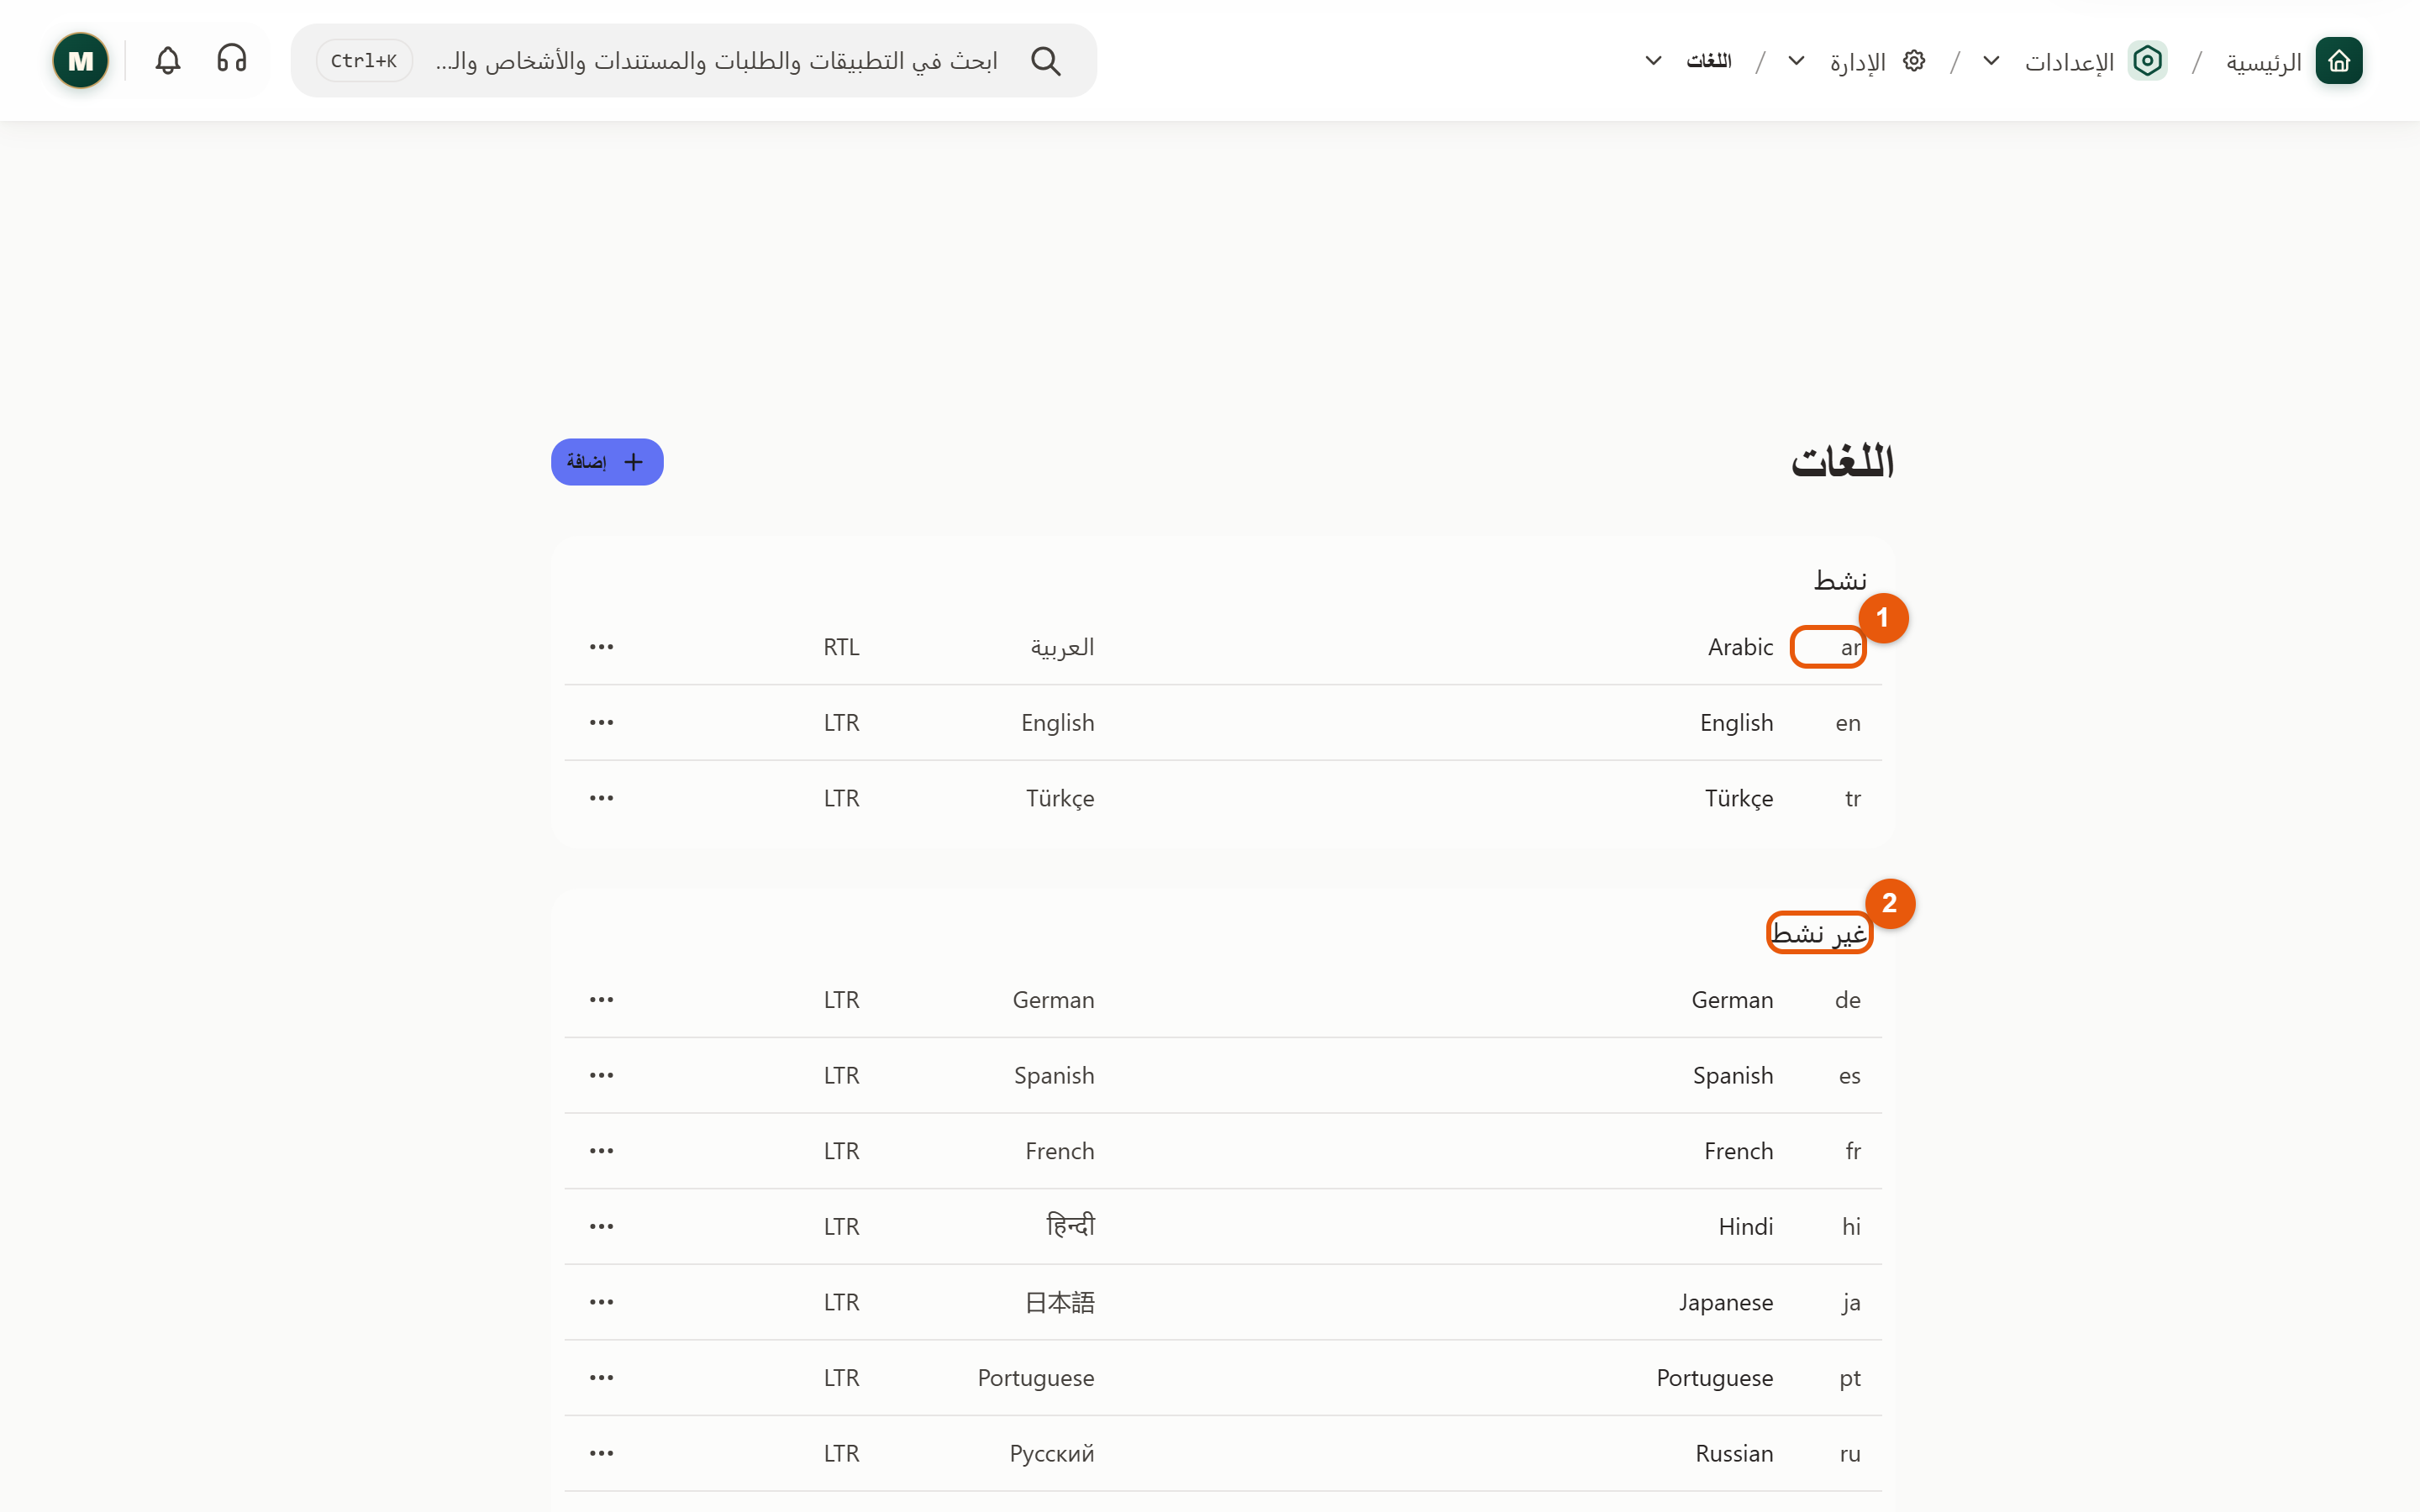
\includegraphics[width=0.95\linewidth]{assets/screens/languages.png}
\caption{لغات المؤسسة}
\label{fig:features-languages}
\shotnote{تحدد الصفحة اللغات المتاحة. ولا توجد «عربية سورية» مستقلة؛ فالعربية لغة واحدة، أما طابعها المحلي فيأتي من أسماء الأشهر والمنطقة الزمنية والعملة. ① اللغة العربية نشطة ورمزها \en{ar}. ② «غير نشط»: لغات لا يراها الأعضاء إلى أن تفعّلها.}
\end{figure}

\subsection{خطوات العمل والتحقق}
\begin{enumerate}
\item افتح «الإعدادات» ← «إعدادات المؤسسة»، واضبط البنود الثلاثة، ثم احفظ.
\item افتح «الإعدادات» ← «اللغات»، وتأكد من أن العربية نشطة.
\end{enumerate}

\textbf{تحقق:} أنشئ تكليفاً تجريبياً بموعد محدد، وتأكد من ظهور اليوم والساعة كما تتوقع. وإذا اختلف الموعد، فراجع المنطقة الزمنية أولاً.

\section{اختر أسماء الأشهر}
\label{sec:features-months}

يدعم كيان أسماء الأشهر المستخدمة في بلاد الشام، مثل «كانون الثاني» و«تشرين الثاني». وتحفظ المؤسسة هذا الخيار لرسائل المتعاملين، فتصل التواريخ إليهم بالأسماء التي يعرفونها.

\begin{rcnote}[مثال: مديرية الواحة]
تختار المديرية الأسماء الشامية، فتصل إلى صاحب «فرن السنابل» رسالة موعد الكشف بتاريخ «الأحد، 8 تشرين الثاني 2026»، لا «8 نوفمبر».
\end{rcnote}

\begin{figure}[H]
\centering
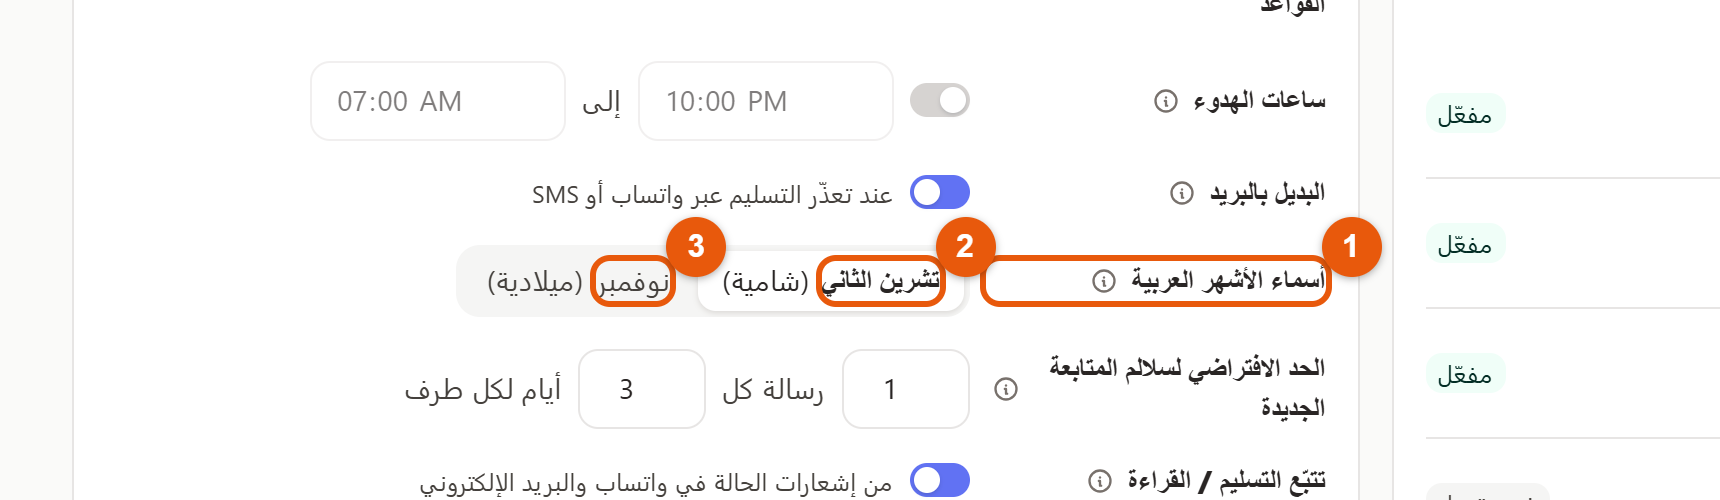
\includegraphics[width=0.9\linewidth]{assets/screens/messages-months.png}
\caption{«أسماء الأشهر العربية»}
\label{fig:features-months}
\shotnote{يقع الخيار في قواعد الرسائل، ويسري على الرسائل المرسلة إلى المتعاملين. ① «أسماء الأشهر العربية». ② «تشرين الثاني (شامية)»: الخيار المناسب في سورية. ③ «نوفمبر (ميلادية)»: للمتعاملين الذين يستخدمون الأسماء الميلادية.}
\end{figure}

وإذا احتجت إلى اسم الفترة داخل حقل محسوب، فاستخدم الدالة \en{periodLabel}. والأسماء الشامية هي الافتراضية فيها، كما يبيّن الجدول التالي. واستبدل \en{visit\_date} بمفتاح حقل التاريخ عندك.

\begin{table}[H]
\centering
\caption{تعبيرات اسم الفترة}
\label{tab:features-period}
\begin{tabularx}{\linewidth}{Y R{3.8cm}}
\rcHeaderRow
\thh{التعبير} & \thh{النتيجة}\\
\srcs{periodLabel(\$.visit\_date, "month", "ar")} & «تشرين الثاني 2026»\\
\srcs{periodLabel(\$.visit\_date, "month", "ar", "gregorian")} & «نوفمبر 2026»\\
\end{tabularx}
\end{table}

\textbf{تحقق:} افتح «الإعدادات» ← «الرسائل» ← «القنوات والقواعد»، وتأكد من تحديد «تشرين الثاني (شامية)». ثم أرسل رسالة تجريبية إلى نفسك، واقرأ التاريخ فيها.

\section{سجّل المبالغ بالليرة السورية}
\label{sec:features-currency}

الحقل الرقمي بتنسيق «نقدي» يعرض كل مبلغ بعملة الحقل، مهما كانت القيمة المكتوبة. فإذا تُركت العملة الافتراضية، ظهر مبلغ بالليرة كأنه بالدولار، وأصبح الفرق بين حقلين بعملتين مختلفين بلا معنى.

\begin{rcnote}[مثال: مديرية الواحة]
ترد شكوى من أن ربطة الخبز بيعت بأربعة آلاف ليرة بدل ألفي ليرة. يجب أن يكون «السعر المدفوع» و«السعر النظامي» بالعملة نفسها، حتى يعني «الفرق» ألفي ليرة فعلاً.
\end{rcnote}

\begin{figure}[H]
\centering
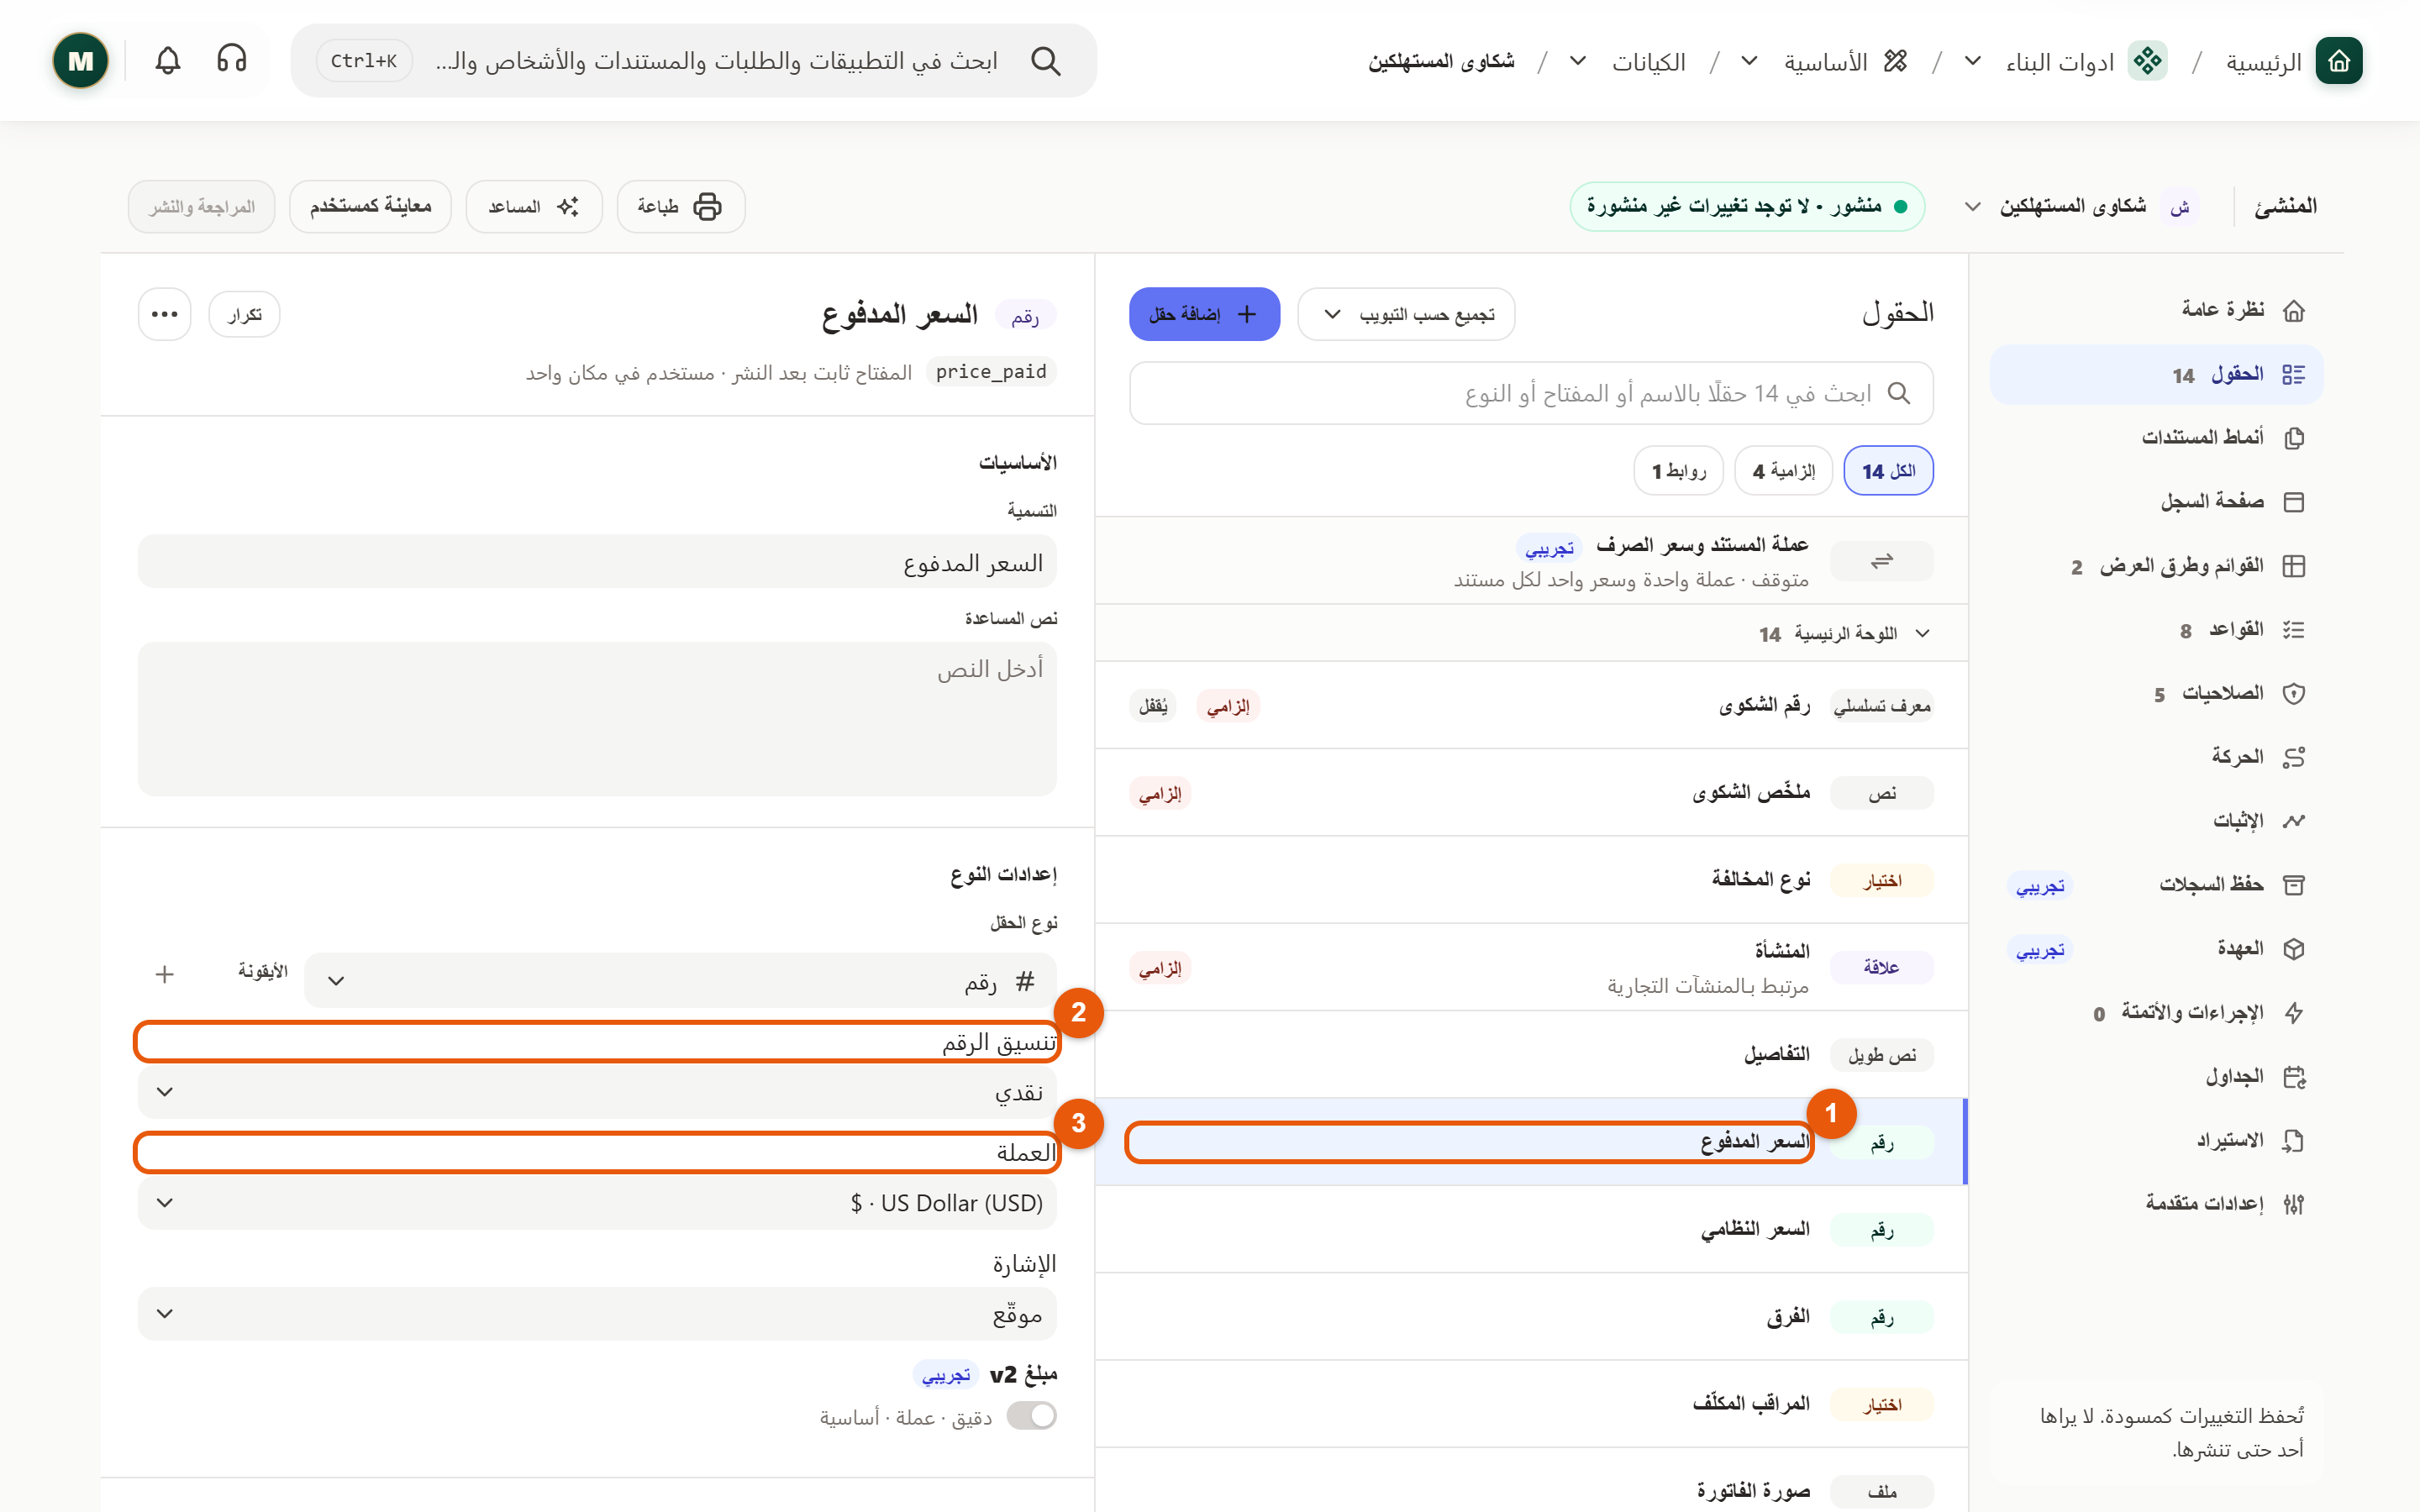
\includegraphics[width=0.95\linewidth]{assets/screens/entity-currency.png}
\caption{عملة الحقل النقدي}
\label{fig:features-currency}
\shotnote{تظهر الصورة حقلاً نقدياً ضُبطت عملته على الدولار الأمريكي، وهو ما يجب تغييره في مثال الليرة. ① الحقل المحدد في قائمة الحقول. ② «تنسيق الرقم»: «نقدي» يعرض المبلغ بعملة. ③ «العملة»: اختر الليرة السورية \en{(SYP)}.}
\end{figure}

\subsection{خطوات العمل والتحقق}
\begin{enumerate}
\item افتح «الكيانات»، ثم نوع السجلات، ثم «الحقول».
\item حدّد كل حقل مبلغ، واجعل «العملة» الليرة السورية. وإذا لم تجدها، فأضفها أولاً من «الإعدادات» ← «العملات».
\item اضغط «المراجعة والنشر».
\end{enumerate}

\textbf{تحقق:} افتح سجلاً، وتأكد من أن المبلغين يظهران بالعملة نفسها وأن «الفرق» صحيح. وإذا كان السجل قديماً، فراجع قيمه؛ فتغيير العملة يغيّر طريقة عرض الرقم فقط، ولا يحوّل قيمته.

\section{اربط الشكاوى بالمنشآت}
\label{sec:features-complaints}

تصبح زيارة الكشف أوضح عندما يرى الباحث شكاوى المنشأة. لذلك أنشئ نوع سجلات للشكاوى، واربطه بالمنشأة بحقل «علاقة»، فتجتمع الشكاوى والكشوف حول سجل واحد.

\begin{table}[H]
\centering
\caption{حقول مقترحة لسجل الشكوى}
\label{tab:features-complaint-fields}
\begin{tabularx}{\linewidth}{R{3.6cm} Y}
\rcHeaderRow
\thh{الحقل} & \thh{نوعه وسببه}\\
«رقم الشكوى» & معرف تسلسلي يولّده النظام، فلا يتكرر رقم.\\
«المنشأة» & علاقة مرتبطة بـ«المنشآت التجارية»، وهي إلزامية.\\
«نوع المخالفة» & اختيار من قائمة، حتى يمكن عدّ المخالفات.\\
«السعر المدفوع» و«السعر النظامي» & حقلان نقديان بالليرة السورية.\\
«الفرق» & حقل يُحسب منهما، فلا يكتبه أحد يدوياً.\\
«صورة الفاتورة» & ملف يثبت الشكوى.\\
«هل نُظّم ضبط؟» و«رقم الضبط» & قيمة منطقية، ويظهر الرقم بشرطها فقط.\\
\end{tabularx}
\end{table}

\begin{rcnote}[مثال: مديرية الواحة]
ترد شكوى عن «فرن السنابل»، فتُربط بسجله. وعندما تفتح ليلى السجل قبل الزيارة، تعرف ما يجب أن تتحقق منه في كشفها.
\end{rcnote}

\begin{figure}[H]
\centering
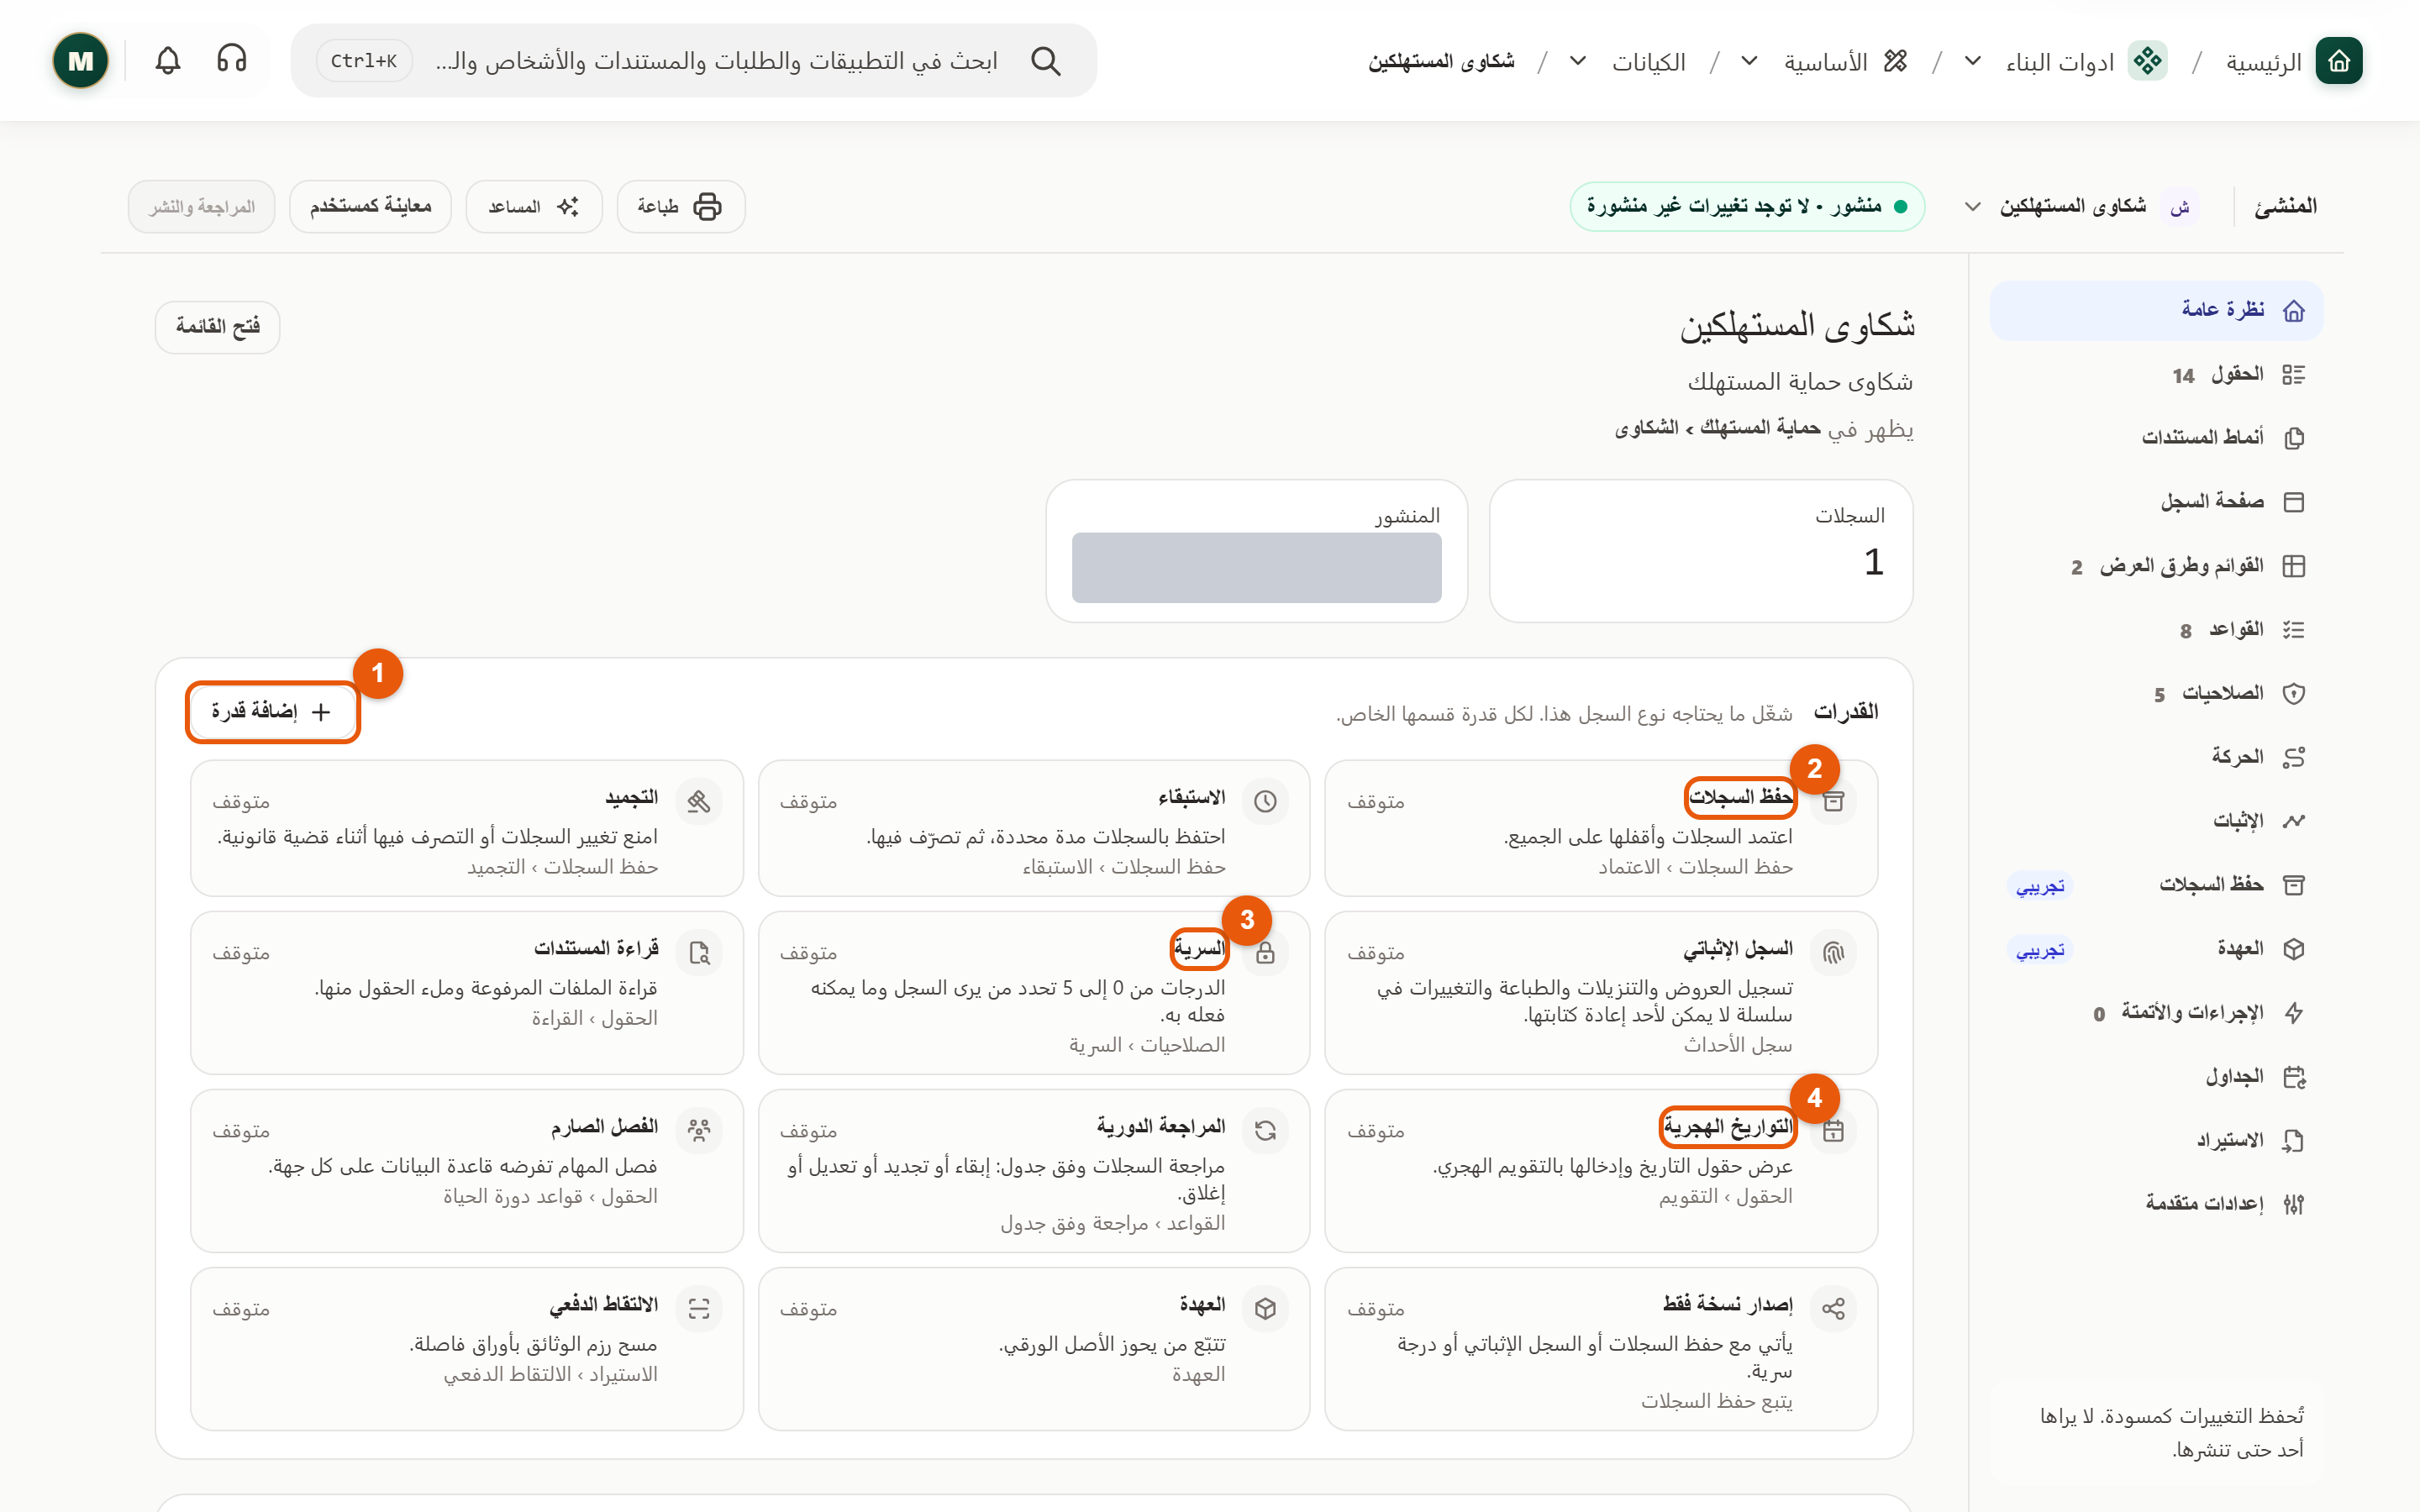
\includegraphics[width=0.95\linewidth]{assets/screens/entity-capabilities.png}
\caption{القدرات الإضافية لنوع السجلات}
\label{fig:features-capabilities}
\shotnote{تجمع «نظرة عامة» قدرات يمكن تشغيلها عند الحاجة، وكلها متوقفة هنا. وهي تضيف قواعد على السجلات، لذلك فعّل ما تحتاجه فقط وجرّبه. ① «إضافة قدرة». ② «حفظ السجلات»: يعتمد السجلات ويقفلها، ويناسب الضبوط النهائية. ③ «السرية»: درجات تحدد من يرى السجل، وتناسب هوية صاحب الشكوى. ④ «التواريخ الهجرية»: لا تحتاجها إذا كانت التواريخ ميلادية.}
\end{figure}

\textbf{تحقق:} افتح سجل المنشأة، وتأكد من ظهور الشكوى المرتبطة به. ثم غيّر «هل نُظّم ضبط؟» إلى نعم، وتأكد من ظهور «رقم الضبط».

\section{اعرض الخدمة على البوابة}
\label{sec:features-services}

يبقى النموذج داخلياً حتى تضمه إلى خدمة. فصفحة «الخدمات» تحدد ما يراه المتعاملون على البوابة، ومن يحق له التقديم، وتضم كل خدمة نموذجاً أو أكثر. ويناسب الكشف البقاء داخلياً، بينما تناسب الشكوى البوابة إذا أرادت الجهة استقبالها من الجمهور.

\begin{rcnote}[مثال: مديرية الواحة]
تبقي المديرية نموذج الكشف داخلياً لأن باحثيها يعبّئونه. وتنشئ خدمة «تقديم شكوى» على البوابة، حتى يصل بلاغ المستهلك مباشرة إلى المديرية.
\end{rcnote}

\begin{figure}[H]
\centering
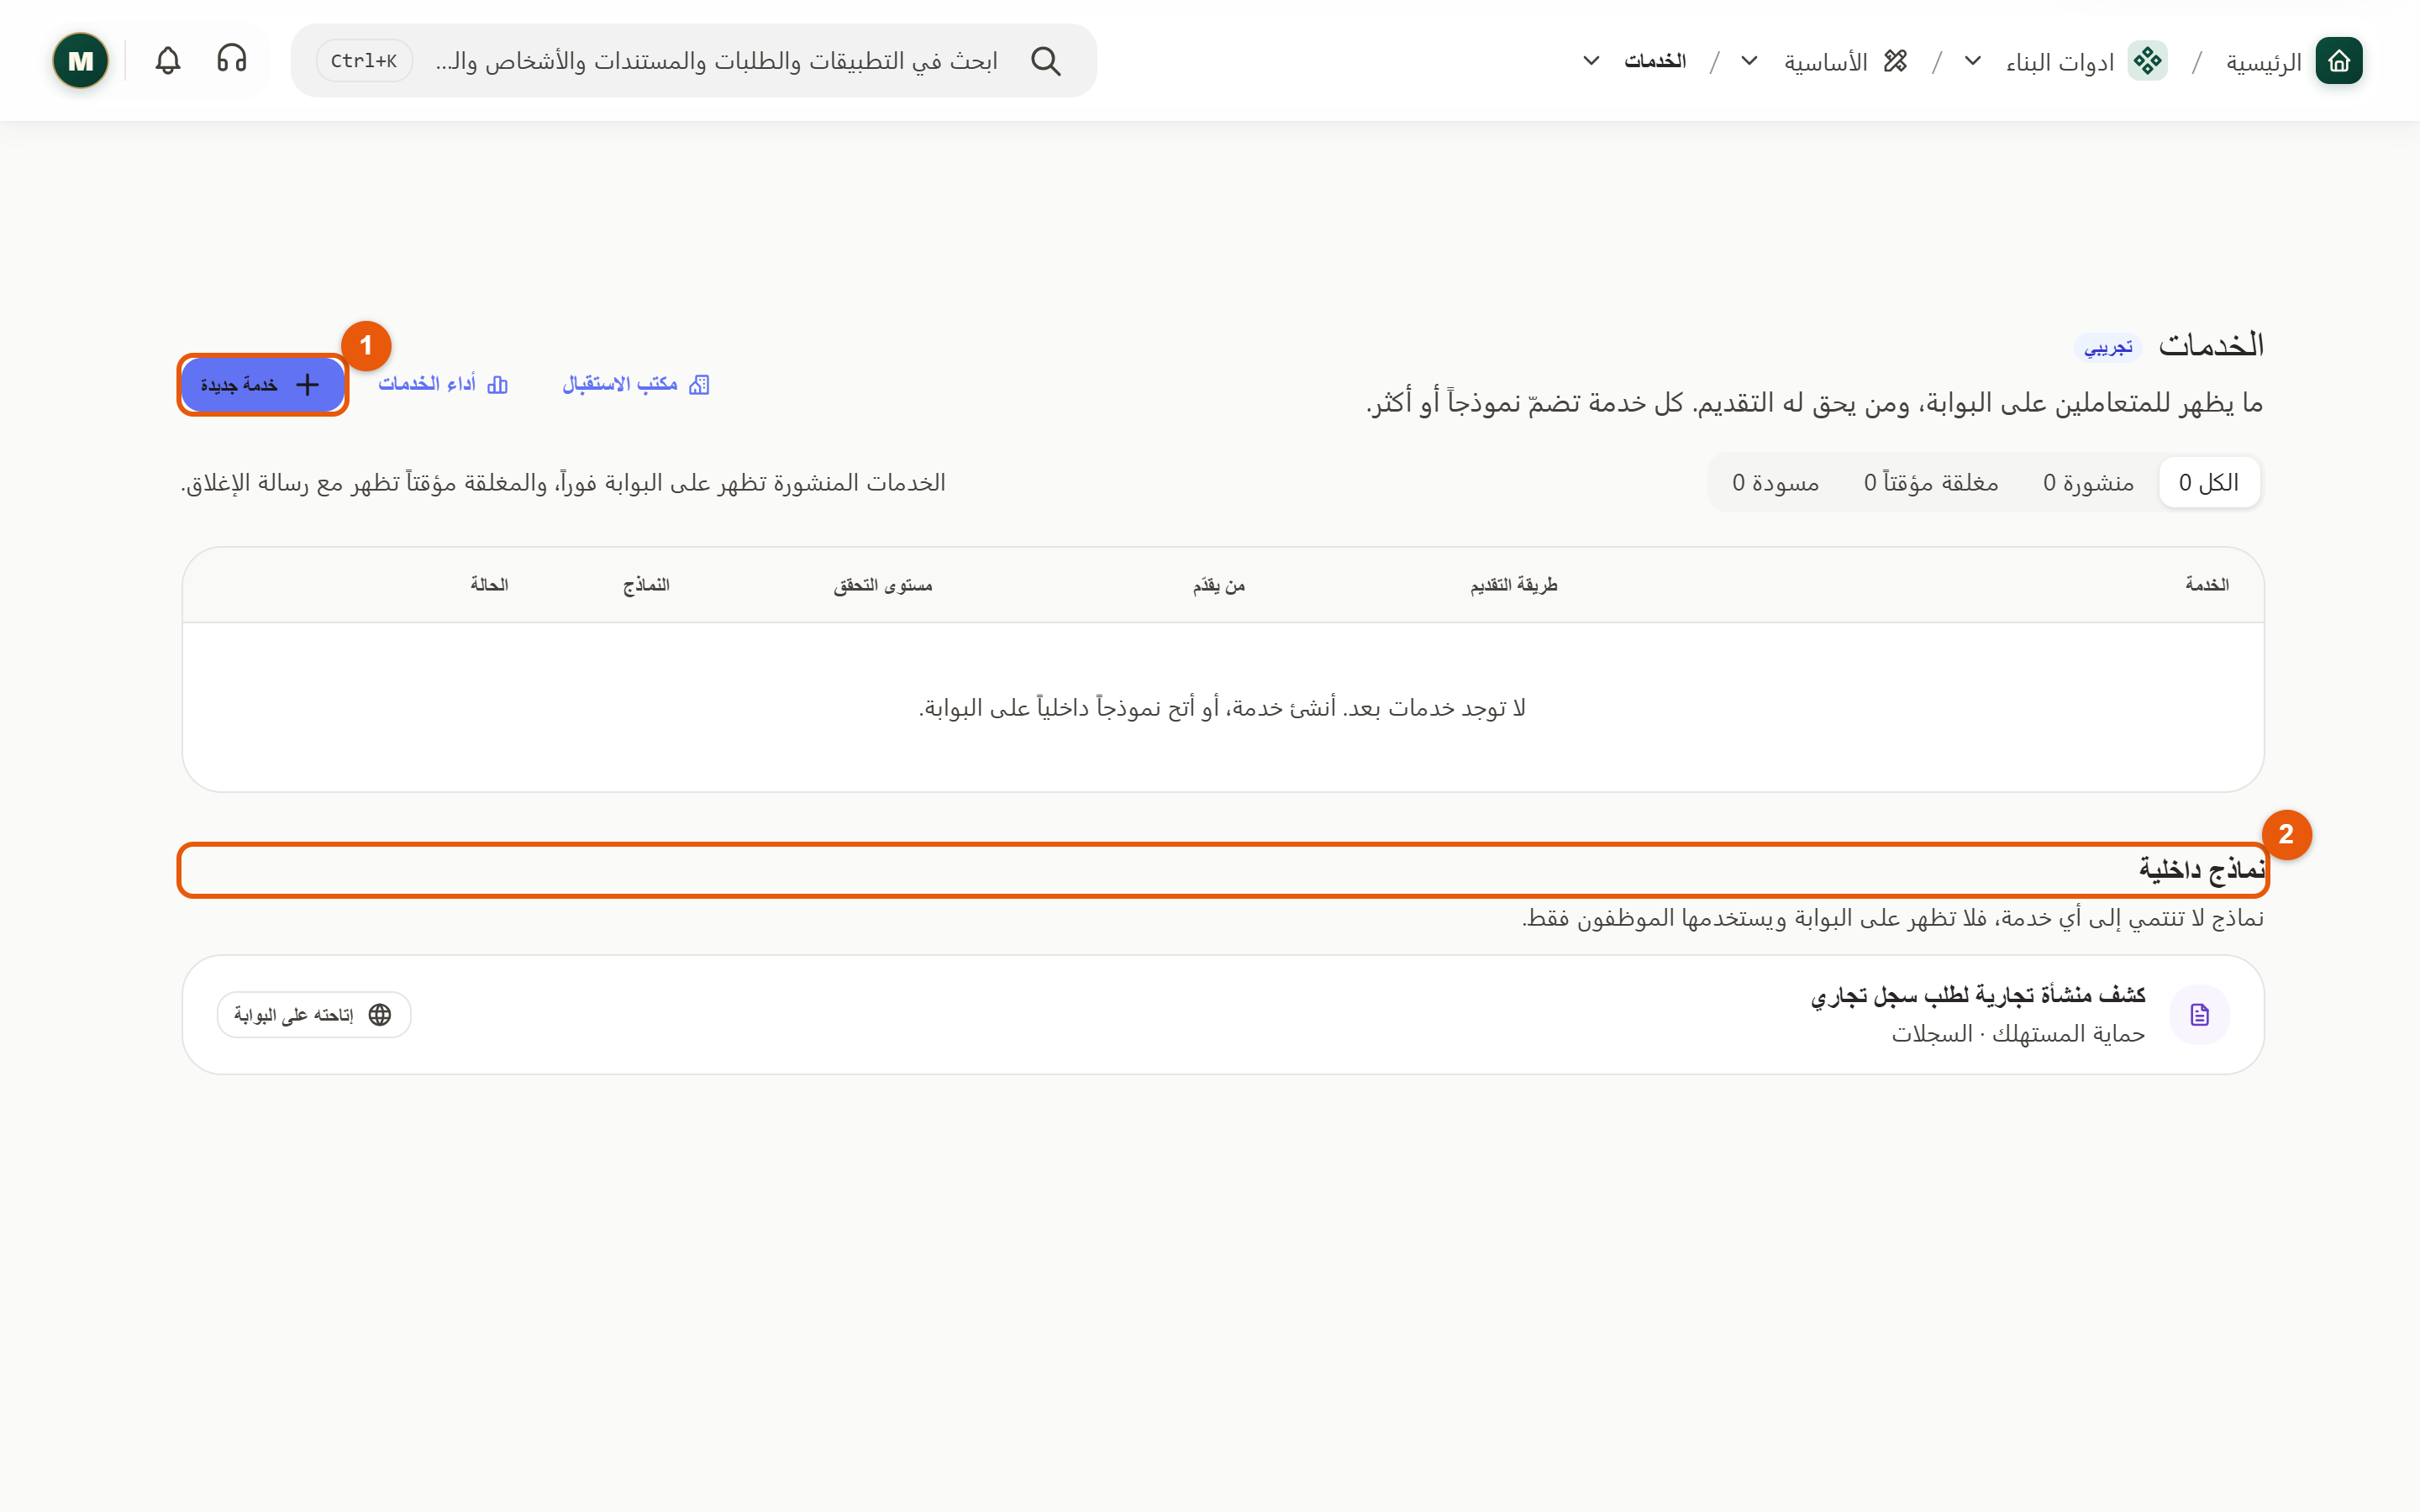
\includegraphics[width=0.95\linewidth]{assets/screens/services.png}
\caption{«الخدمات»}
\label{fig:features-services}
\shotnote{لا توجد في الصورة خدمة منشورة، لذلك لا يظهر شيء للمتعاملين. وتظهر الخدمة المنشورة على البوابة فوراً، فراجعها قبل نشرها. ① «خدمة جديدة». ② «نماذج داخلية»: نماذج لا تنتمي إلى خدمة، ويستخدمها الموظفون فقط.}
\end{figure}

\textbf{تحقق:} افتح البوابة في نافذة خاصة دون تسجيل الدخول، وتأكد من ظهور الخدمة أو عدم ظهورها بحسب ما تريد.

\section{طبّق المثال واختبره}
\label{sec:features-test}

هذا اختبار كامل لما بنيته، ويكشف ما لا يظهر عند فتح الشاشات فقط. نفّذه بحساب باحث وحساب مدقق مختلفين، وعلى منشأة تجريبية يسهل تمييزها وإزالتها بعد الانتهاء.

\begin{rcnote}[مثال: مديرية الواحة]
تضيف المديرية منشأة باسم «تجربة: فرن السنابل» في «المزة»، وتنفذ الاختبارات التالية عليها بالترتيب، ثم تزيل السجل التجريبي.
\end{rcnote}

\begin{table}[H]
\centering
\caption{خطوات الاختبار}
\label{tab:features-test}
\begin{tabularx}{\linewidth}{R{4.6cm} Y}
\rcHeaderRow
\thh{افعل} & \thh{يجب أن ترى}\\
افتح المسار، ثم «الفحص». & لا تحذيرات عن توقيع ناقص أو أزرار تتجاوز الموافقة.\\
كلّف الباحث بالمنشأة من خطة مُطلقة. & تظهر له مهمة واحدة، والمنشأة محددة في الكشف.\\
أرسل الكشف بحساب الباحث. & تصبح الحالة «قيد التدقيق»، ويتوقف تعديله، ويبقى عنوان المنشأة كما كان.\\
اختر «اعتماد الكشف» بحساب المدقق. & تصبح الحالة «مقبول»، وتُكتب الحقول المسموح بها إلى سجل المنشأة.\\
أعد كشفاً ثانياً بخيار «إعادة للتصحيح». & تصبح الحالة «بحاجة إلى تصحيح»، وبعد الإرسال تبدأ جولة جديدة.\\
ارفض كشفاً ثالثاً. & تصبح الحالة «مرفوض»، وتبقى بيانات المنشأة دون تغيير.\\
حاول قبول كشف بحساب الباحث. & لا يظهر له الخيار، ويرفض النظام الإجراء إن حاوله.\\
\end{tabularx}
\end{table}

\begin{rcchecklist}[قائمة تحقق: جاهز للعمل الفعلي]
\begin{checklist}
  \item نجحت خطوات الجدول كلها بحسابين مختلفين.
  \item المبالغ بالليرة السورية، والتواريخ بالمنطقة الزمنية الصحيحة.
  \item سُجّل من اختبر، ومتى، وما النتيجة.
  \item أُزيلت السجلات التجريبية.
\end{checklist}
\end{rcchecklist}
